\documentclass[11pt,a4paper]{article}

\usepackage[a4paper,margin=1in]{geometry}
\usepackage[T1]{fontenc}
\usepackage[utf8]{inputenc}
\usepackage{lmodern}
\usepackage{booktabs}
\usepackage{array}
\usepackage{longtable}
\usepackage{hyperref}
\usepackage{enumitem}
\usepackage{xcolor}
\usepackage{graphicx}
\usepackage{float}
\usepackage{listings}

\lstset{
    basicstyle=\ttfamily\small,
    breaklines=true,
    frame=single,
    columns=fullflexible
}

\hypersetup{
    colorlinks=true,
    linkcolor=blue,
    urlcolor=blue
}

\title{CS305 SDN Project Report}
\author{
    Tong Wu (12412460) \and
    Zhikai Wang (12410615) \and
    Yunzang Li (12410922)
}
\date{\today}

\begin{document}

\maketitle

\section{Introduction}

This project implements a centralized Software-Defined Networking controller using
os-ken and Mininet. The network is modeled as a single-subnet Layer-2 environment with
hosts and OpenFlow switches. Our controller supports three required functions:

\begin{itemize}[leftmargin=1.5em]
    \item dynamic IP allocation through DHCP,
    \item shortest-path forwarding based on the current topology,
    \item traffic filtering through a switch-level firewall.
\end{itemize}

In addition to the required tasks, we also implemented bonus functionality and
experiments, including DNS support, DHCP lease improvements, TCP congestion experiments,
and a bufferbloat study.

\section{Architecture}

The system is built around a centralized controller that maintains the global topology
state and installs OpenFlow rules into switches. Mininet creates the virtual hosts,
switches, and links. Hosts generate traffic, while the controller decides how the network
should react.

The architecture can be described in four layers:

\begin{itemize}[leftmargin=1.5em]
    \item \textbf{Topology and switching layer}: maintains switch, link, and host state;
    computes shortest paths; installs forwarding rules.
    \item \textbf{DHCP layer}: processes DHCP messages and manages IP allocation, pending
    offers, leases, and renewals.
    \item \textbf{Firewall layer}: parses deny rules from the JSON rule file and installs
    high-priority drop flows.
    \item \textbf{Bonus DNS layer}: answers DNS queries according to static DNS records.
\end{itemize}

\subsection{Core Files}

\begin{itemize}[leftmargin=1.5em]
    \item \texttt{controller.py}: main controller logic. It receives switch, host, link,
    port, and packet events; maintains the topology view; handles ARP; delegates DHCP and
    DNS processing; and installs forwarding and firewall rules.
    \item \texttt{dhcp.py}: DHCP server implementation, including allocation, lease
    management, timeout reclaim, and renewal support.
    \item \texttt{firewall.py}: firewall rule parsing and installation logic.
    \item \texttt{dns\_server.py}: bonus DNS implementation.
    \item \texttt{ofctl\_utilis.py}: OpenFlow helper utilities for flow installation,
    packet-out operations, and related switch interaction.
    \item \texttt{tests/}: Mininet-based validation scripts for required and bonus parts.
\end{itemize}

\subsection{Control Logic}

The controller maintains the following shared state:

\begin{itemize}[leftmargin=1.5em]
    \item online datapaths and OpenFlow control abstractions,
    \item learned hosts and IP-to-MAC mappings,
    \item switch adjacency information,
    \item inter-switch output port mappings,
    \item down-port information used for topology refresh.
\end{itemize}

The forwarding logic is built on top of this global view. Once host locations and switch
links are known, the controller computes shortest paths and installs destination-MAC-based
flow rules on the relevant switches.

\subsection{Representative Code Snippets}

The following simplified snippets illustrate the core implementation ideas.

\paragraph{DHCP address reservation and reclaim.}
\begin{lstlisting}[language=Python]
def allocate_ip(client_mac):
    reclaim_expired_leases()
    if client_mac in ip_pool:
        return ip_pool[client_mac]
    if client_mac in pending_offers:
        return pending_offers[client_mac]["ip"]
    for ip in build_ip_range():
        if ip not in in_use_ips() and ip not in bad_ips:
            pending_offers[client_mac] = {
                "ip": ip,
                "timestamp": now(),
            }
            return ip
    return None
\end{lstlisting}

\paragraph{Shortest-path forwarding refresh.}
\begin{lstlisting}[language=Python]
for src_mac, src_info in hosts.items():
    for dst_mac, dst_info in hosts.items():
        if src_mac == dst_mac:
            continue
        path = shortest_path(src_info["dpid"], dst_info["dpid"])
        for dpid in path:
            out_port = next_hop_port(dpid, path, dst_info["port"])
            install_dst_mac_flow(dpid, dst_mac, out_port)
\end{lstlisting}

\paragraph{Firewall deny-rule installation.}
\begin{lstlisting}[language=Python]
for dpid, ofctl in ofctls.items():
    for rule in rules:
        if rule.action != "deny":
            continue
        ofctl.set_flow(
            priority=60000,
            dl_type=IP,
            nw_src=rule.src_ip or 0,
            nw_dst=rule.dst_ip or 0,
            nw_proto=proto_to_number(rule.proto),
            tp_src=normalize_port(rule.src_port),
            tp_dst=normalize_port(rule.dst_port),
            actions=[],
        )
\end{lstlisting}

\section{Implementation Details}

\subsection{DHCP}

The DHCP module implements the standard DISCOVER/OFFER/REQUEST/ACK workflow. Hosts are
created without valid initial IP addresses in the test scripts, so IP allocation must be
handled by the controller.

The implementation in \texttt{dhcp.py} keeps track of:

\begin{itemize}[leftmargin=1.5em]
    \item pending offers,
    \item confirmed leases,
    \item lease expiration timestamps,
    \item rejected addresses that should not be reused.
\end{itemize}

We also extended the baseline DHCP design with practical improvements:

\begin{itemize}[leftmargin=1.5em]
    \item configurable address pool and netmask,
    \item offer timeout reclaim,
    \item lease expiration and renewal support,
    \item conflict-free allocation under concurrent requests.
\end{itemize}

\subsection{Topology Learning and Shortest-Path Switching}

The switching part is implemented in \texttt{controller.py}. The controller:

\begin{itemize}[leftmargin=1.5em]
    \item learns hosts through gratuitous ARP and ARP requests,
    \item learns switch-to-switch links through LLDP and topology APIs,
    \item updates internal topology state on switch, host, link, and port events,
    \item computes shortest paths on the switch graph using breadth-first search,
    \item installs destination-MAC forwarding rules on the switches.
\end{itemize}

This design supports both the basic triangle topology and complex topologies with loops
and dynamic changes.

\subsection{Firewall}

The firewall module reads policy rules from \texttt{firewall\_rule.json}. Each rule can
match source IP, destination IP, transport protocol, source port, and destination port.
The module converts each deny rule into a high-priority OpenFlow drop flow.

The firewall rules are installed on every switch through \texttt{Firewall.install\_rules}.
Since the firewall rules have higher priority than normal forwarding rules, they override
shortest-path forwarding whenever traffic matches a deny rule.

\subsection{Bonus Components}

\paragraph{DNS.}
The DNS bonus extends the controller with a controller-hosted DNS service. DNS requests
are detected in \texttt{controller.py} and answered according to static records defined in
\texttt{dns\_records.json}.

\paragraph{TCP Congestion.}
The TCP congestion bonus is an experiment built with Mininet rather than a controller-side
feature. It compares TCP algorithms such as Reno and Cubic under the same bottleneck and
reports throughput and fairness.

\paragraph{Bufferbloat.}
The bufferbloat bonus is another Mininet experiment. It studies the tradeoff between
throughput and queueing delay under different queue sizes.

\section{Team Division of Work}

We adopted a module-oriented collaboration strategy: each member took long-term ownership
of a subsystem and the team merged changes continuously during development.

\begin{longtable}{>{\raggedright\arraybackslash}p{0.24\textwidth} >{\raggedright\arraybackslash}p{0.45\textwidth} >{\raggedright\arraybackslash}p{0.23\textwidth}}
\toprule
\textbf{Member} & \textbf{Main Responsibilities} & \textbf{Key Files} \\
\midrule
\endfirsthead
\toprule
\textbf{Member} & \textbf{Main Responsibilities} & \textbf{Key Files} \\
\midrule
\endhead
Tong Wu (12412460)\\Role A: DHCP \& Bonus DHCP &
DHCP basic workflow, lease management, duplicate allocation prevention, DHCP option
handling, and DHCP-related testing &
\texttt{dhcp.py}, \texttt{tests/dhcp\_test/}, bonus DHCP scripts \\
\midrule
Zhikai Wang (12410615)\\Role B: Topology \& Switching &
Topology event handling, ARP processing, shortest-path computation, forwarding rule
installation, dynamic topology updates, and switching complex case design &
\texttt{controller.py}, \texttt{ofctl\_utilis.py}, \texttt{tests/switching\_test/},
complex topology scripts \\
\midrule
Yunzang Li (12410922)\\Role C: Firewall \& Report/Experiment &
Firewall rule loading and installation, experiment bonuses, report organization, figures,
screenshots, and demonstration script support &
\texttt{firewall.py}, \texttt{firewall\_rule.json}, \texttt{tests/firewall\_test/},
\texttt{report/} and experiment scripts \\
\bottomrule
\end{longtable}

\section{Testing Methodology}

We used Mininet-based scripts to validate both baseline functionality and complex dynamic
scenarios. The main required tests are grouped into three categories.

\subsection{DHCP Tests}

\begin{itemize}[leftmargin=1.5em]
    \item Basic DHCP allocation with default configuration.
    \item Custom DHCP configuration with modified \texttt{start\_ip}, \texttt{end\_ip},
    and \texttt{netmask}.
    \item Address pool exhaustion where the number of hosts exceeds the pool size.
    \item Bonus DHCP tests for lease timeout reclaim, concurrent allocation, lease
    expiration, and renewal.
\end{itemize}

\begin{figure}[H]
    \centering
    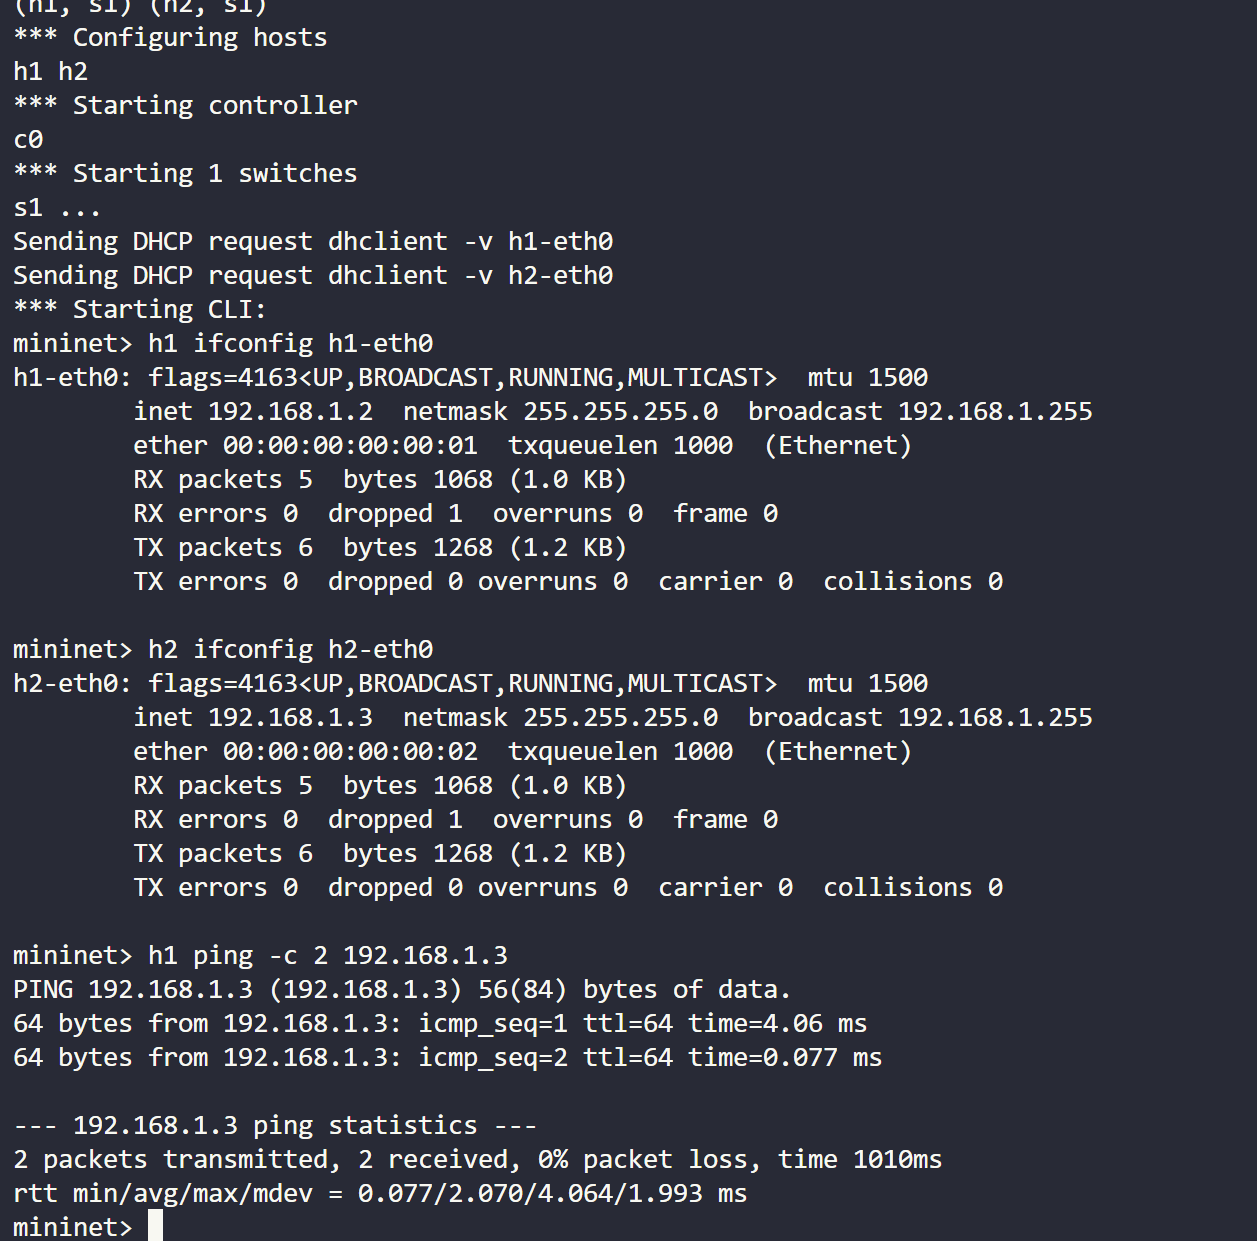
\includegraphics[width=0.62\textwidth]{img/dhcp_basic_result.png}
    \caption{Basic DHCP validation showing successful IP assignment and connectivity.}
\end{figure}

\begin{figure}[H]
    \centering
    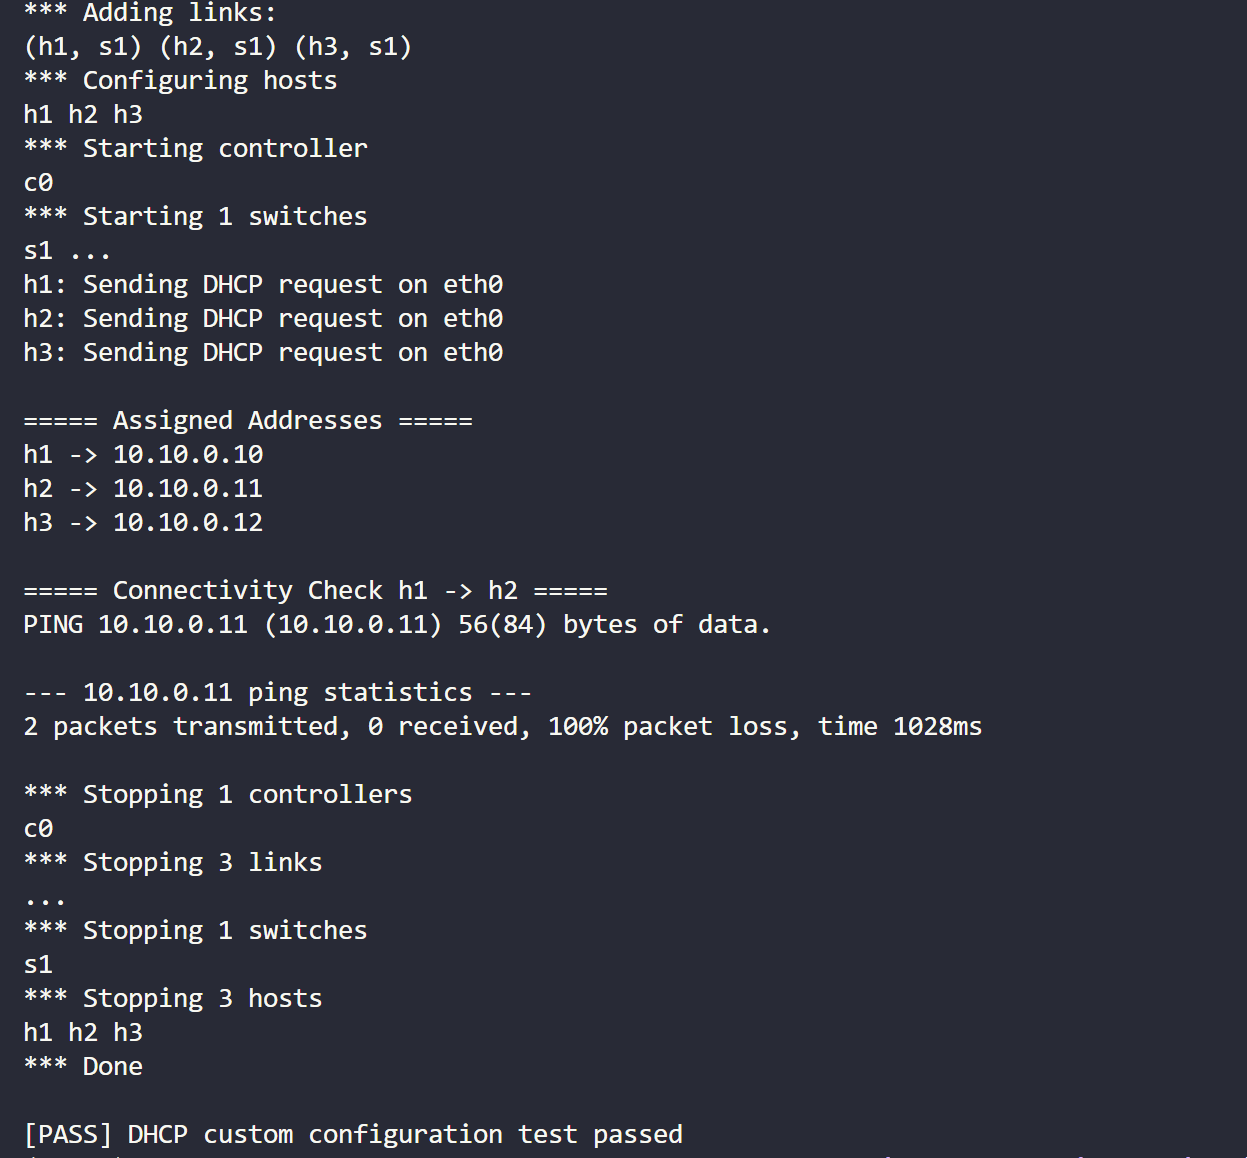
\includegraphics[width=0.62\textwidth]{img/dhcp_custom_result.png}
    \caption{Custom DHCP configuration test with modified address pool and subnet mask.}
\end{figure}

\begin{figure}[H]
    \centering
    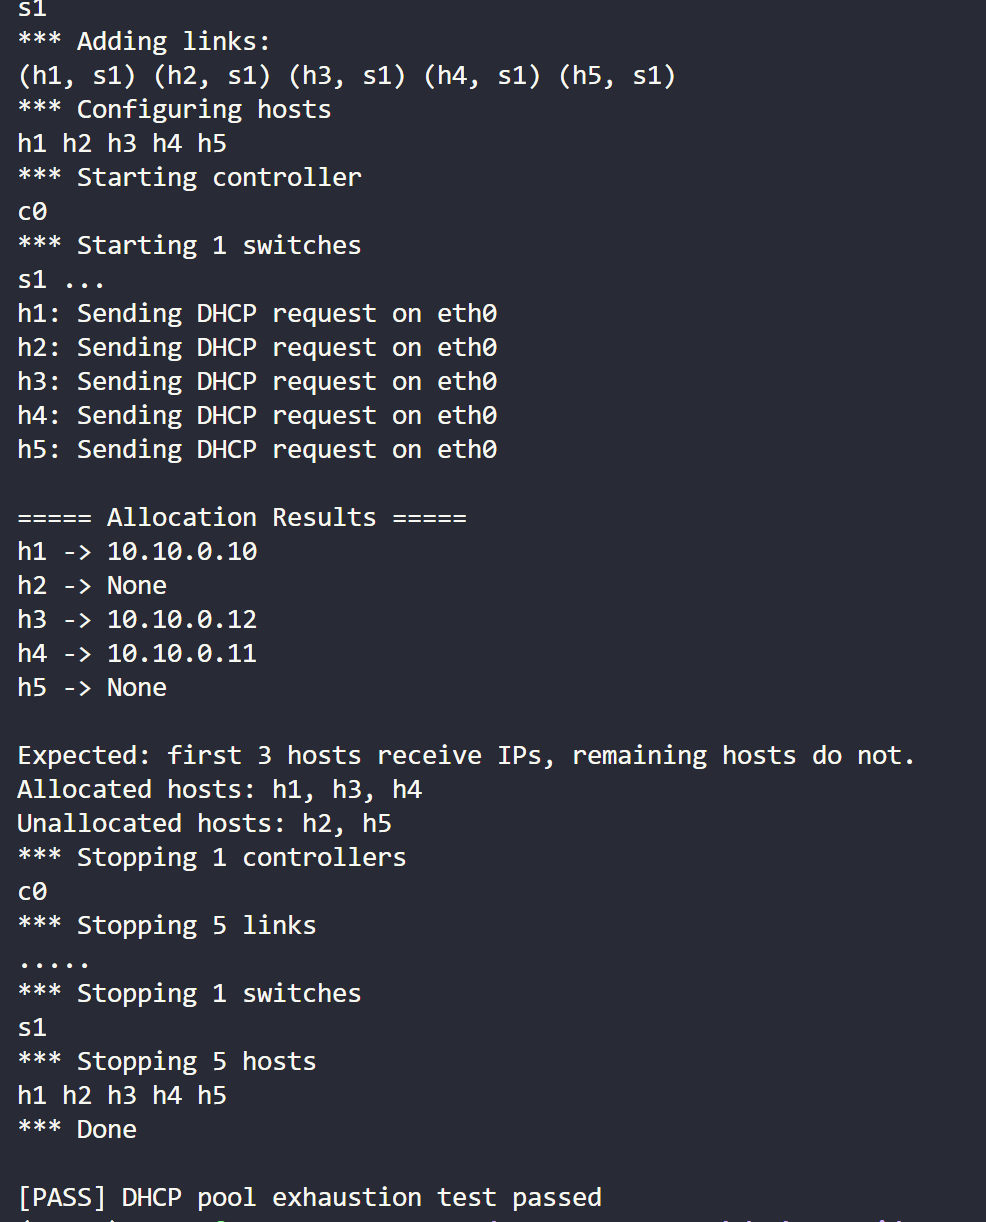
\includegraphics[width=0.55\textwidth]{img/dhcp_pool_exhaustion.png}
    \caption{Pool exhaustion test where only the first hosts receive addresses.}
\end{figure}

\subsection{Shortest-Path Switching Tests}

\begin{itemize}[leftmargin=1.5em]
    \item Basic triangle topology with full host reachability.
    \item Complex topology with more than 6 hosts, more than 6 switches, and more than
    10 edges.
    \item Dynamic topology changes including link down/up, switch stop/start, and port
    disable/enable.
\end{itemize}

\begin{figure}[H]
    \centering
    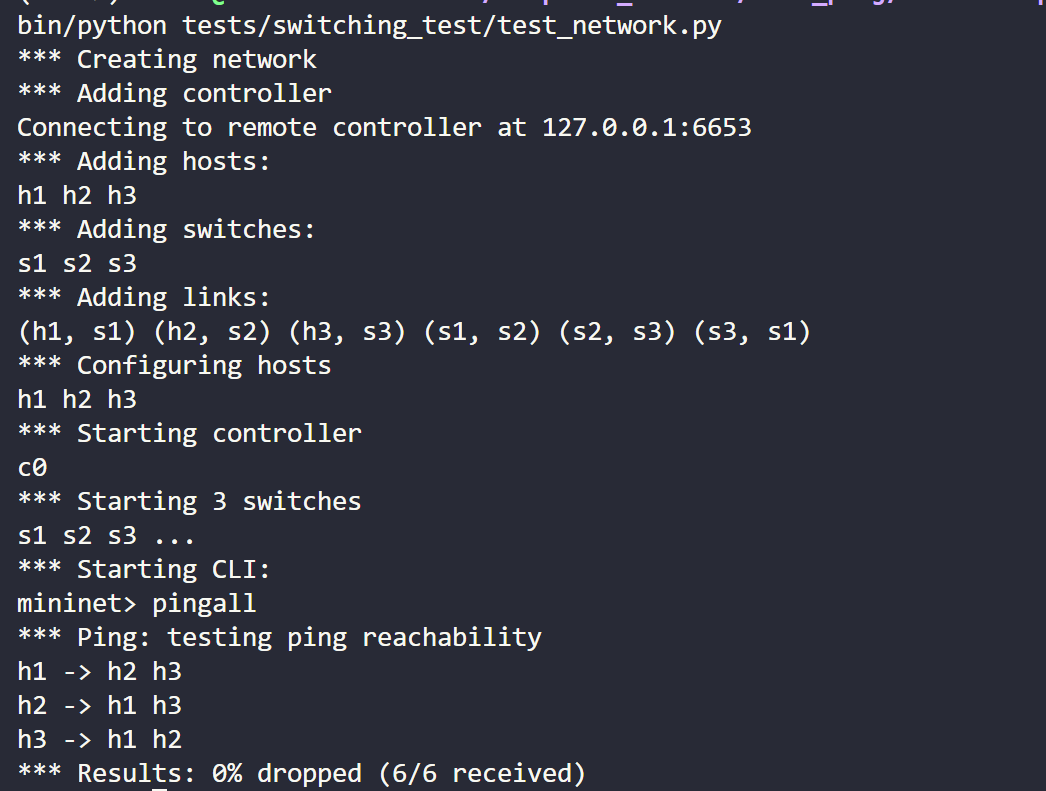
\includegraphics[width=0.56\textwidth]{img/switching_basic_pingall.png}
    \caption{Basic switching result in the triangle topology.}
\end{figure}

\subsection{Firewall Tests}

\begin{itemize}[leftmargin=1.5em]
    \item Basic firewall policy enforcement in a single-switch topology.
    \item Complex multi-switch firewall case reusing the switching complex topology.
    \item Verification that previously reachable hosts become unreachable when firewall
    rules are installed, while unrelated traffic remains allowed.
\end{itemize}

\begin{figure}[H]
    \centering
    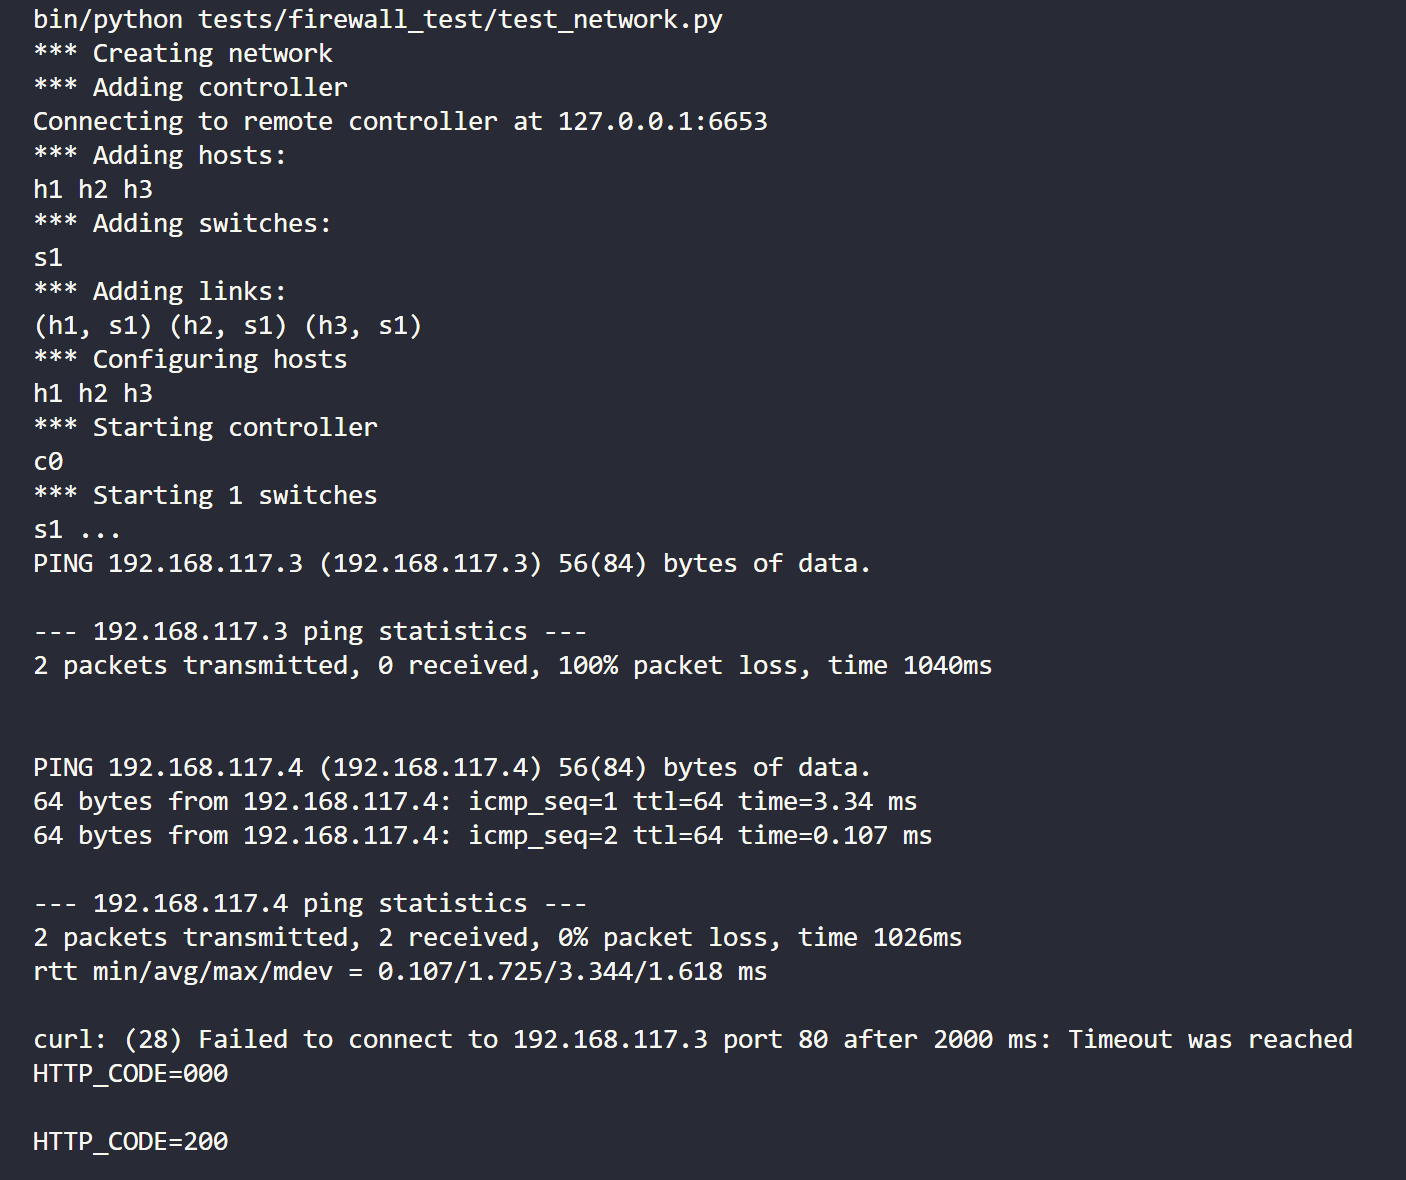
\includegraphics[width=0.78\textwidth]{img/firewall_basic.png}
    \caption{Basic firewall validation results.}
\end{figure}

\begin{figure}[H]
    \centering
    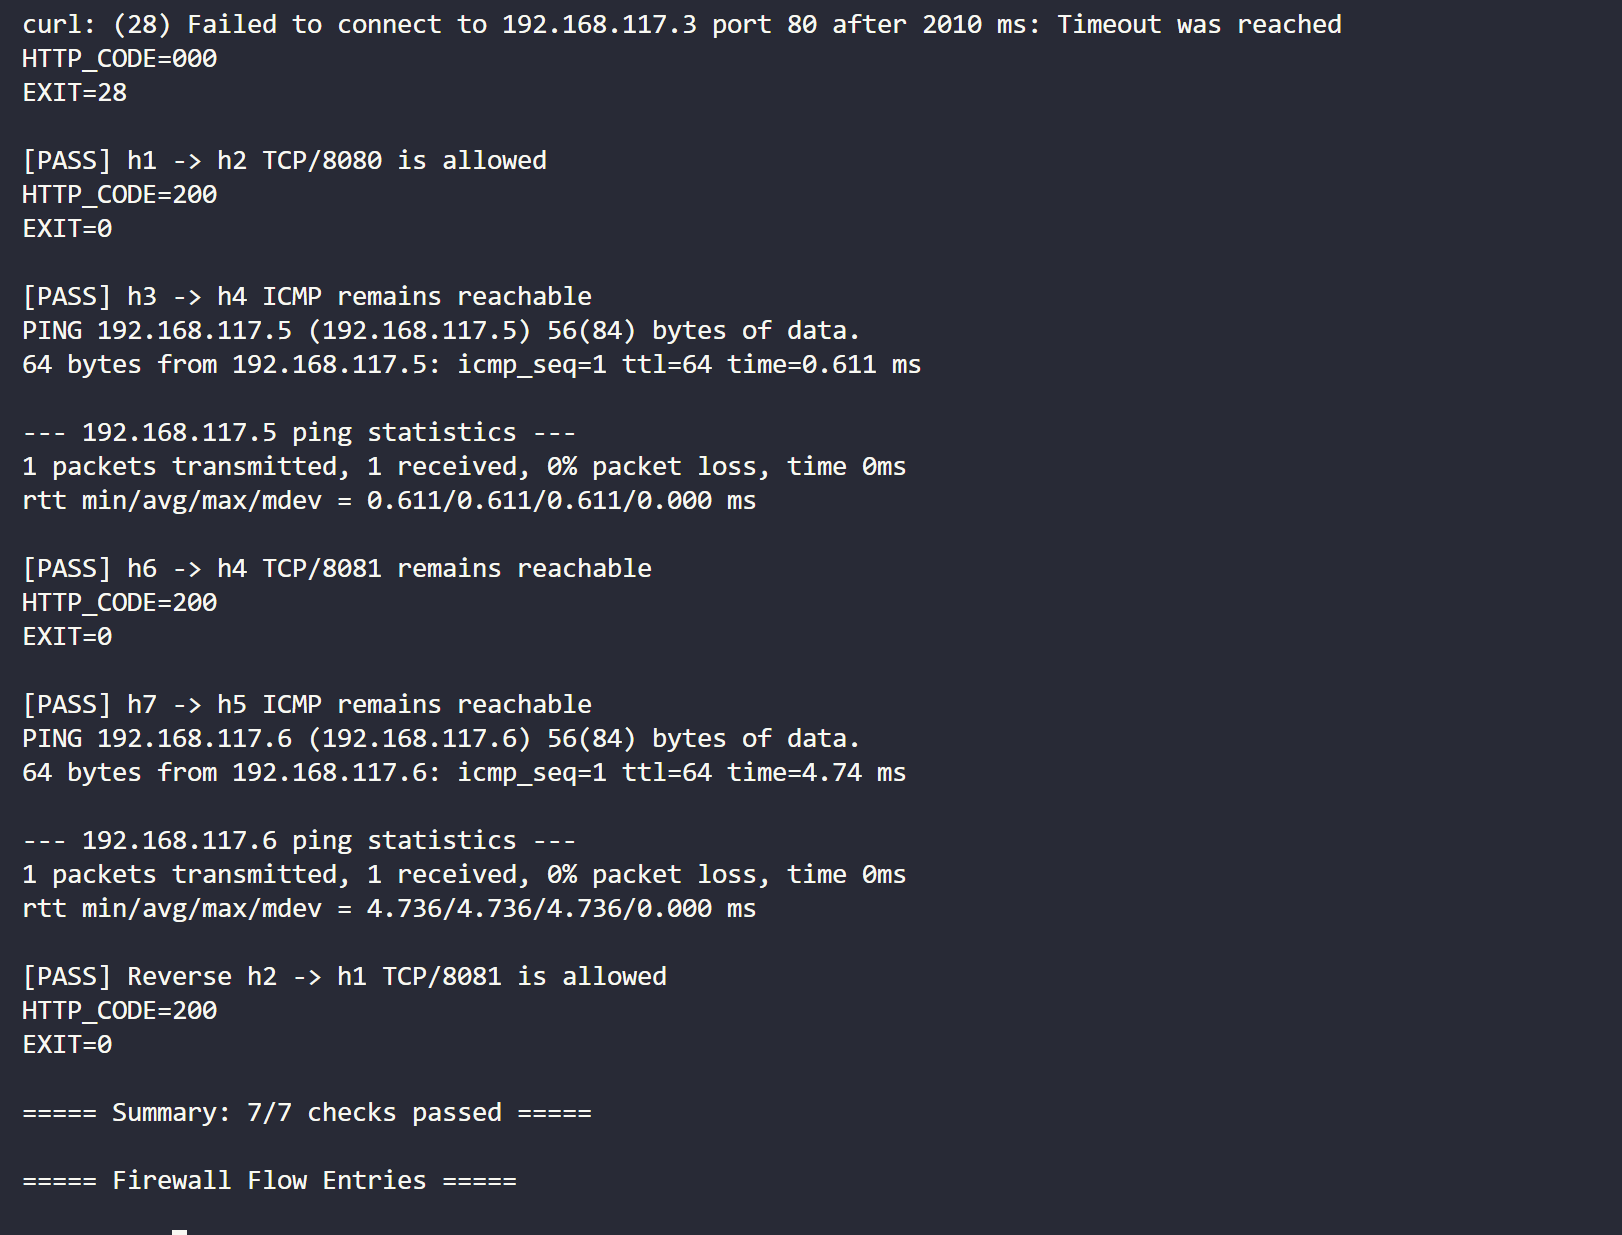
\includegraphics[width=0.72\textwidth]{img/firewall_complex_result.png}
    \caption{Complex firewall validation results.}
\end{figure}

\section{Complex Test Case}

The project instructions explicitly require a complex topology with more than 6 hosts,
more than 6 switches, and more than 10 edges. We designed such a topology and used it in
both the switching and firewall demonstrations.

\subsection{Topology Summary}

\begin{itemize}[leftmargin=1.5em]
    \item Hosts: 7
    \item Switches: 7
    \item Inter-switch edges: 12
\end{itemize}

The complete Mermaid version of the topology and the host-to-host shortest path table are
documented in \texttt{docs/complex-case-topology.md}.

\begin{figure}[H]
    \centering
    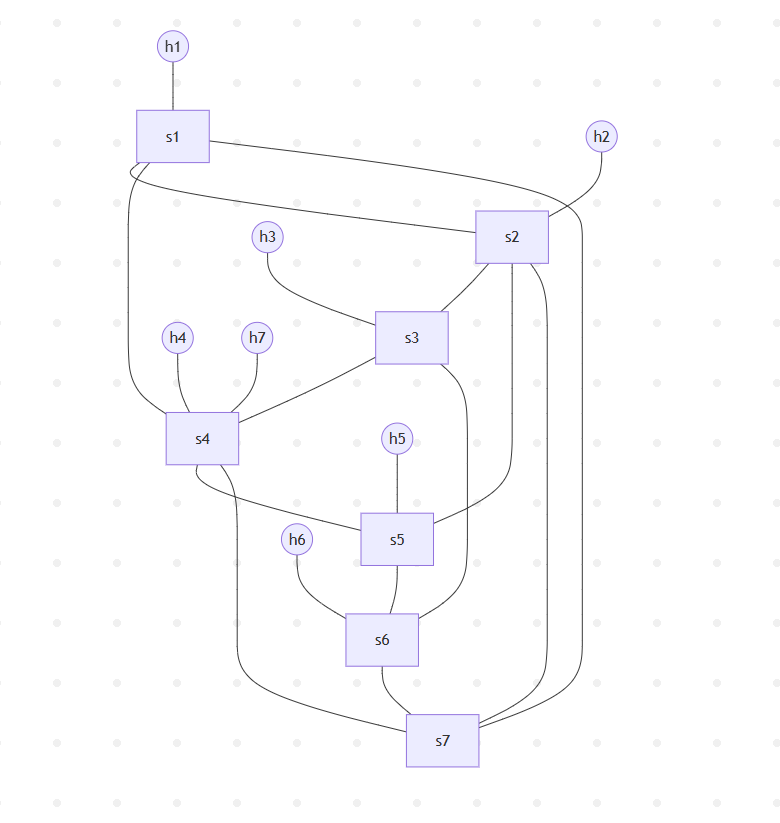
\includegraphics[width=0.42\textwidth]{img/switching_complex_topo.png}
    \caption{Complex topology used in the extended demonstration.}
\end{figure}

\subsection{Dynamic Operations}

The complex case supports dynamic operations from the Mininet CLI:

\begin{itemize}[leftmargin=1.5em]
    \item link down/up,
    \item switch stop/start,
    \item port down/up through \texttt{ovs-ofctl mod-port}.
\end{itemize}

These operations are used to demonstrate that the controller can adapt its forwarding
rules when the topology changes.

\begin{figure}[H]
    \centering
    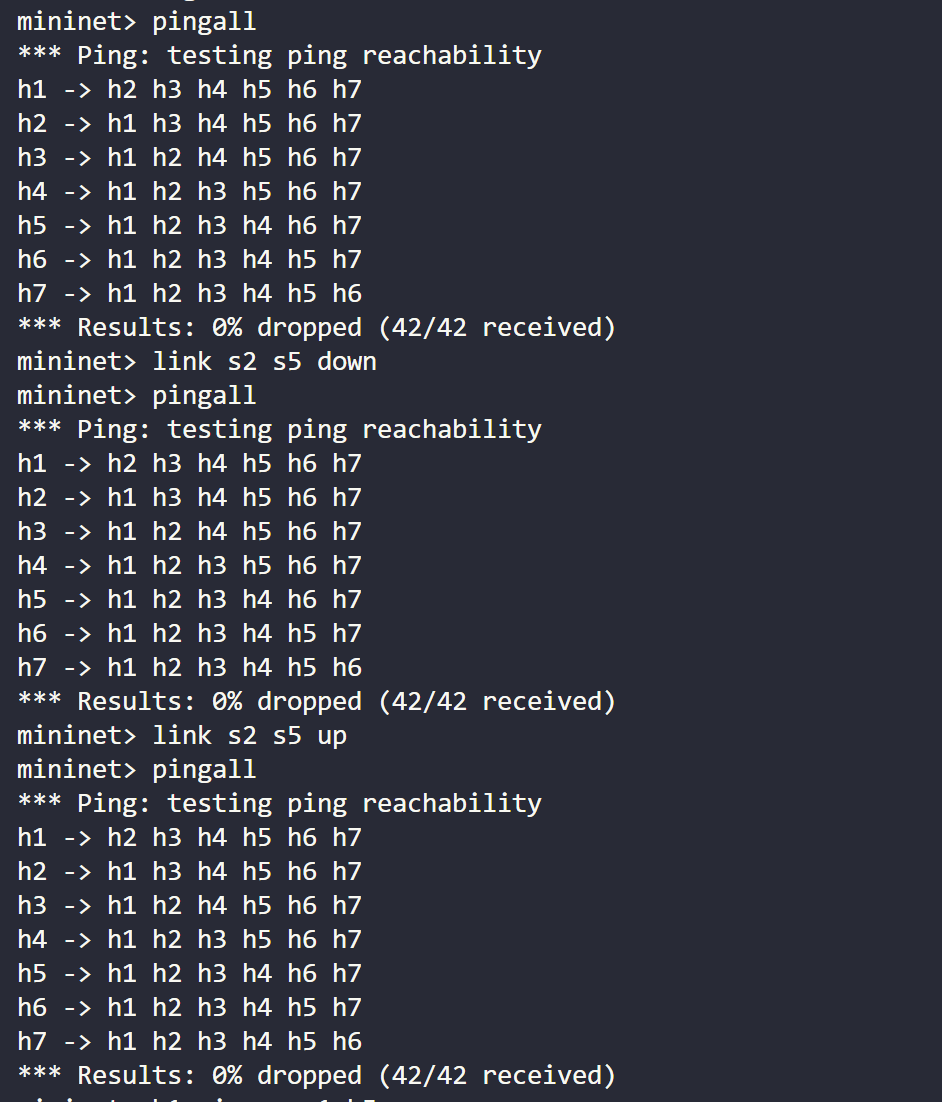
\includegraphics[width=0.55\textwidth]{img/switching_complex_controller_paths.png}
    \caption{Connectivity validation during dynamic topology change operations in the complex case.}
\end{figure}

\section{Bonus Results and Analysis}

\subsection{DNS Bonus}

The DNS bonus demonstrates that the controller can also act as a simple DNS responder.
This shows that the same SDN controller can host protocol logic beyond DHCP and forwarding.

\begin{figure}[H]
    \centering
    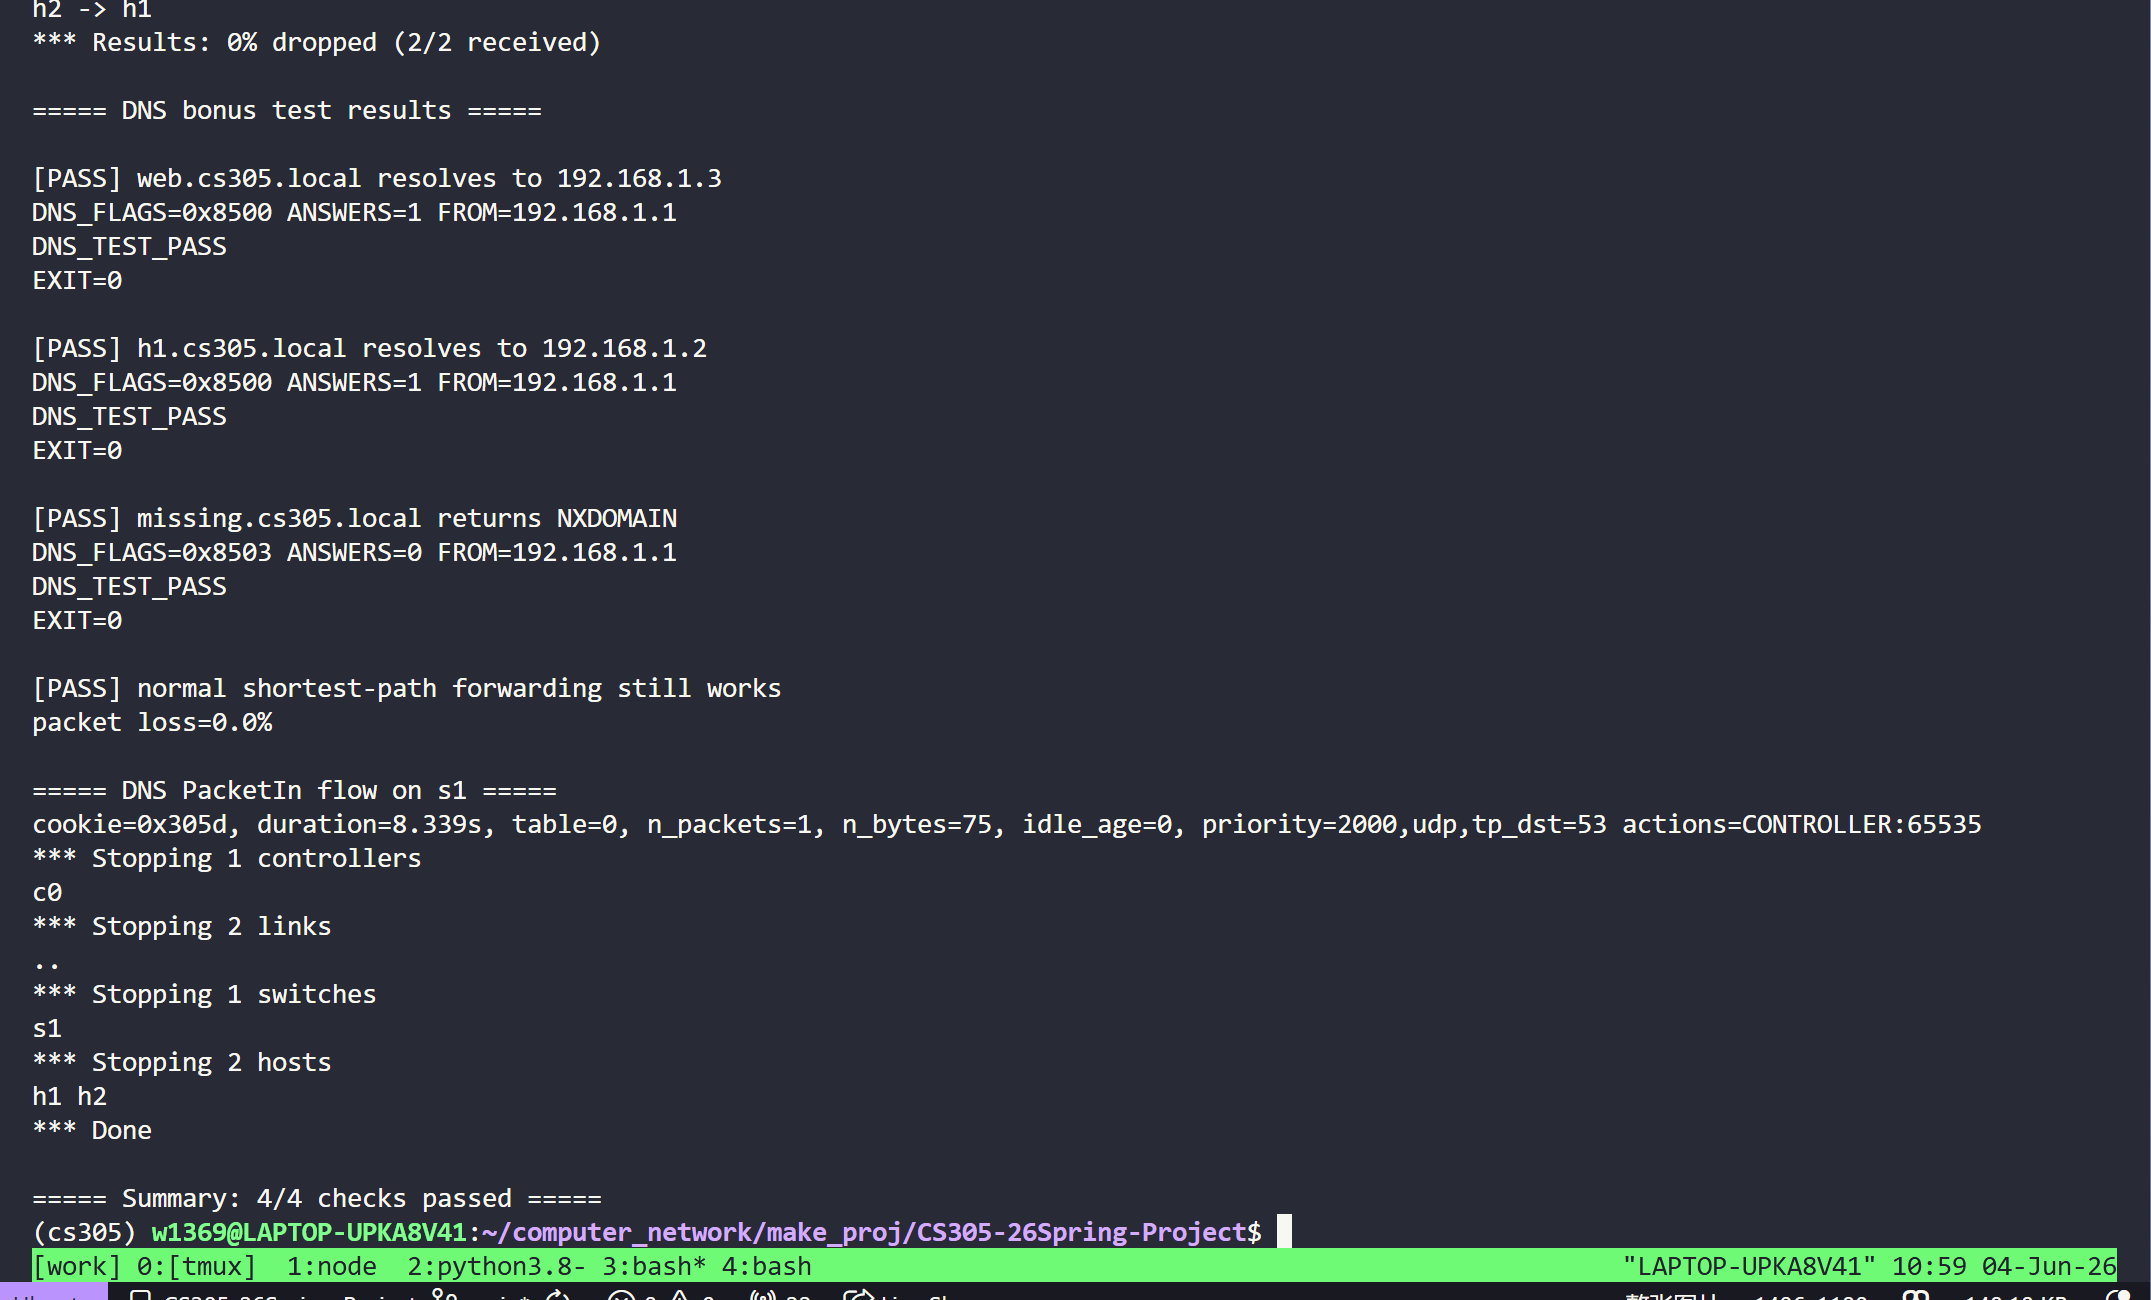
\includegraphics[width=0.78\textwidth]{img/dns_test.png}
    \caption{DNS bonus test results.}
\end{figure}

\subsection{TCP Congestion Bonus}

The TCP congestion experiment compares algorithm behavior under the same bottleneck.
Our results show that the different algorithms produce different throughput values, while
fairness remains close to 1 in the shared-flow scenario.

\begin{figure}[H]
    \centering
    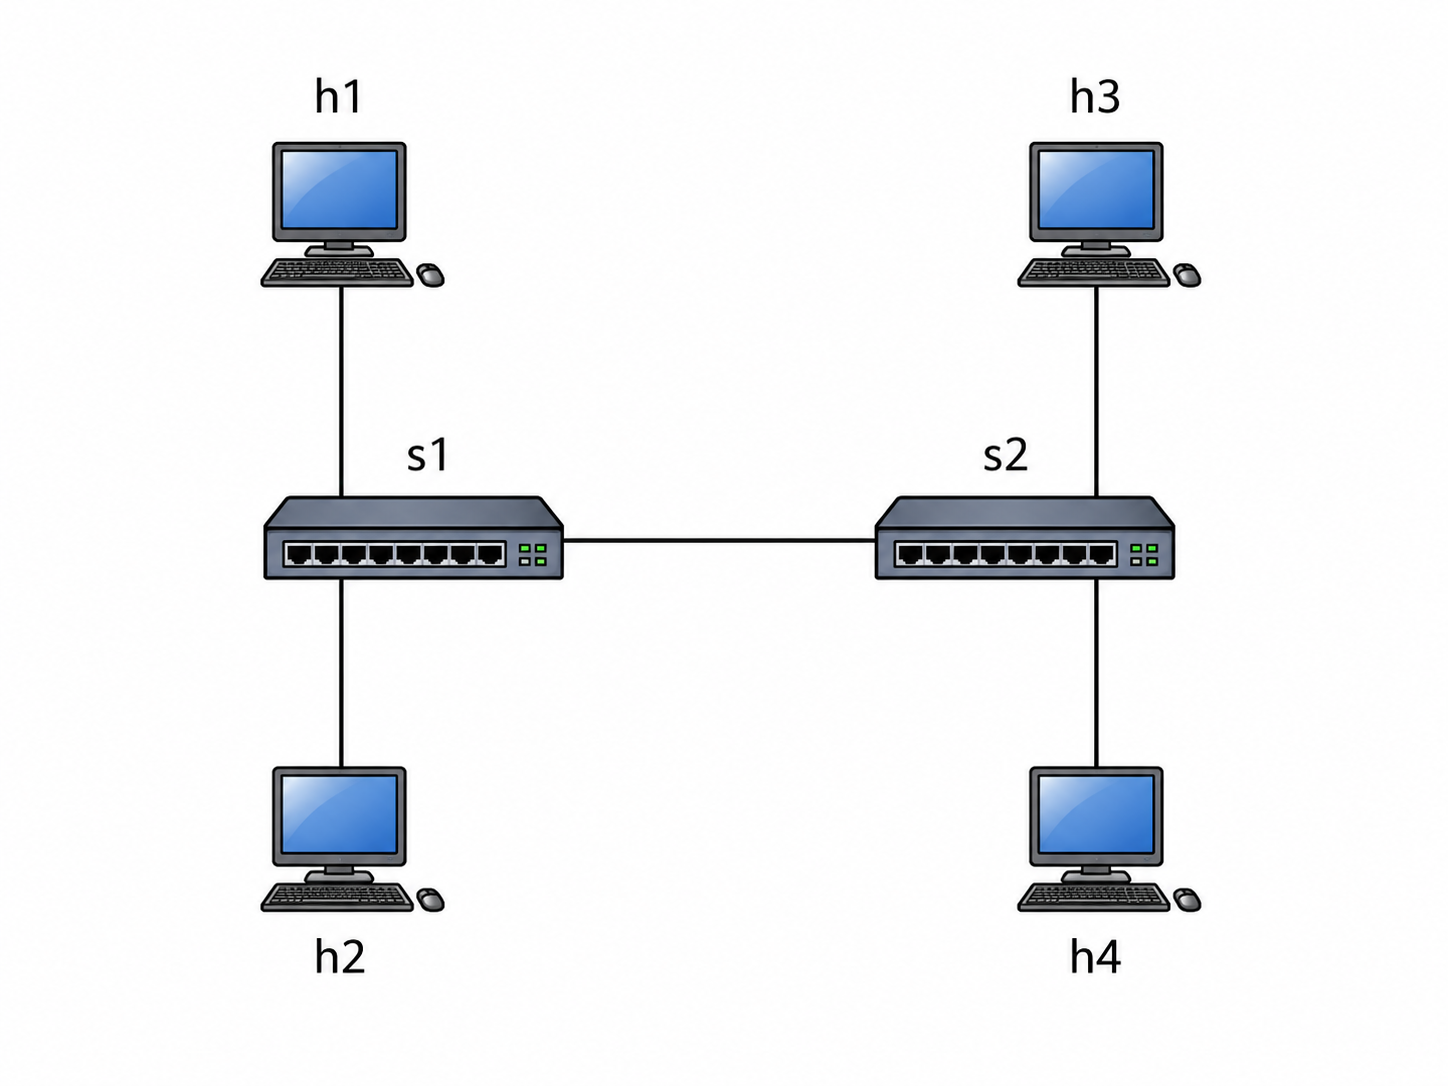
\includegraphics[width=0.72\textwidth]{img/bonus5_topo.png}
    \caption{Mininet topology used in the TCP congestion and bufferbloat bonus experiments.}
\end{figure}

\begin{figure}[H]
    \centering
    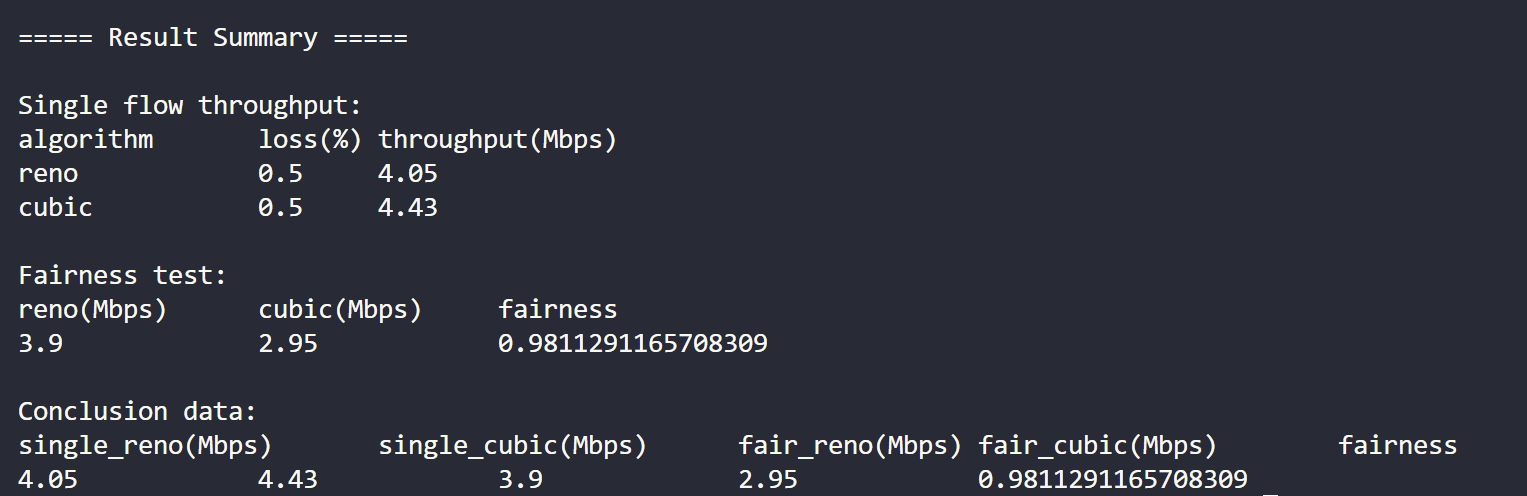
\includegraphics[width=0.82\textwidth]{img/tcp_congestion.png}
    \caption{TCP congestion experiment results for Reno, CUBIC, and the fairness test.}
\end{figure}

\subsection{Bufferbloat Bonus}

The bufferbloat experiment shows the classic tradeoff between throughput and delay.
With a very large queue, packet loss can decrease and throughput can improve, but the
busy RTT becomes much larger, which clearly demonstrates queueing delay inflation.

\begin{figure}[H]
    \centering
    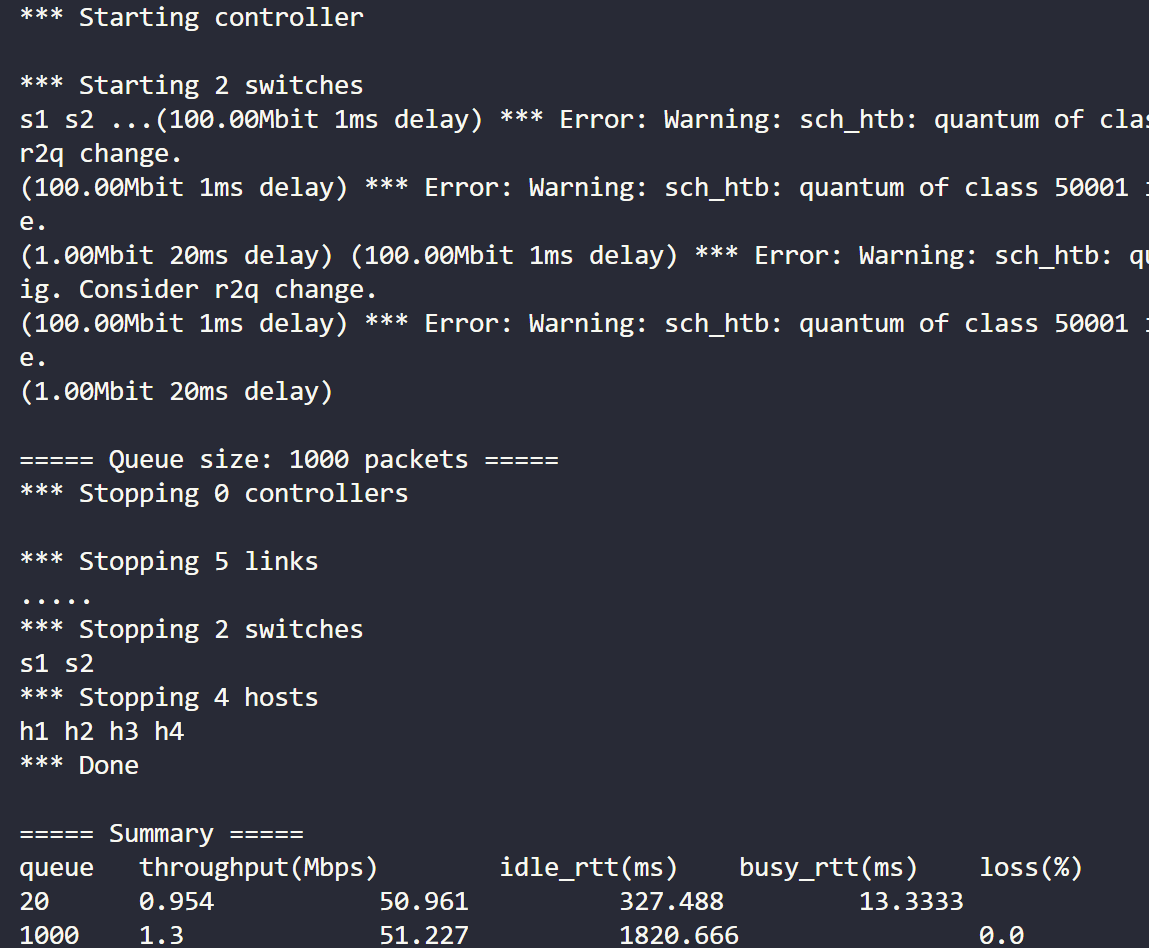
\includegraphics[width=0.82\textwidth]{img/bufferbloat.png}
    \caption{Bufferbloat experiment results comparing small and large bottleneck queues.}
\end{figure}

\section{Conclusion}

This project delivers a functional SDN controller that combines DHCP, shortest-path
switching, and firewall enforcement in one os-ken application. The implementation is
supported by Mininet-based testing, a complex topology for robustness demonstration, and
bonus experiments that extend both protocol functionality and network measurement depth.

The final report should be read together with the test scripts and demo documents in the
repository, especially the complex topology documentation and the defense guide.

\end{document}
